\documentclass[tikz,border=8pt]{standalone}
\usepackage{amsmath,amssymb}
\usetikzlibrary{arrows.meta,calc}

\begin{document}
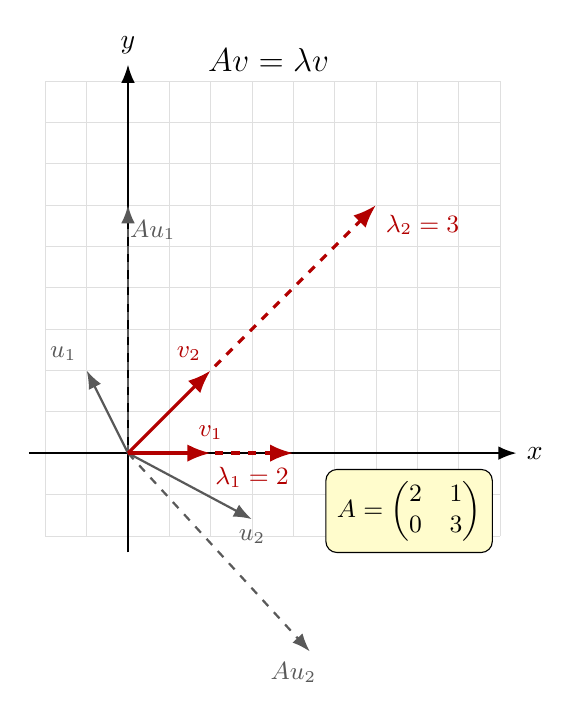
\begin{tikzpicture}[>=Latex, scale=1.05]
  % light grid
  \draw[step=0.5, gray!25, very thin] (-1.0, -1.0) grid (4.5, 4.5);

  % axes
  \draw[->, thick] (-1.2, 0) -- (4.7, 0) node[right]{$x$};
  \draw[->, thick] (0, -1.2) -- (0, 4.7) node[above]{$y$};

  % Ordinary vector u1 = (-0.5, 1.0); A*u1 = (-1+1, 0+3) = (0, 3)
  \draw[->, thick, gray!70!black] (0, 0) -- (-0.5, 1.0) node[above left, font=\small]{$u_1$};
  \draw[->, thick, gray!70!black, dashed] (0, 0) -- (0, 3.0);
  \node[font=\small, gray!70!black] at (0.3, 2.7) {$Au_1$};

  % Ordinary vector u2 = (1.5, -0.8); A*u2 = (3 - 0.8, 0 - 2.4) = (2.2, -2.4)
  \draw[->, thick, gray!70!black] (0, 0) -- (1.5, -0.8) node[below, font=\small]{$u_2$};
  \draw[->, thick, gray!70!black, dashed] (0, 0) -- (2.2, -2.4);
  \node[font=\small, gray!70!black] at (2.0, -2.65) {$Au_2$};

  % Eigenvector v1 = (1, 0), λ=2
  \draw[->, very thick, red!70!black] (0, 0) -- (1, 0);
  \draw[->, very thick, red!70!black, dashed] (1.05, 0) -- (2, 0);
  \node[font=\small, red!70!black, anchor=south] at (1, 0.05) {$v_1$};
  \node[font=\small, red!70!black, anchor=north] at (1.5, -0.05) {$\lambda_1=2$};

  % Eigenvector v2 = (1, 1), λ=3
  \draw[->, very thick, red!70!black] (0, 0) -- (1, 1);
  \draw[->, very thick, red!70!black, dashed] (1.05, 1.05) -- (3, 3);
  \node[font=\small, red!70!black, anchor=south east] at (1, 1) {$v_2$};
  \node[font=\small, red!70!black, anchor=north west] at (3, 3) {$\lambda_2=3$};

  % Matrix label
  \node[draw, fill=yellow!20, rounded corners, font=\small, inner sep=4pt] at (3.4, -0.7)
    {$A=\begin{pmatrix}2 & 1\\ 0 & 3\end{pmatrix}$};

  % Equation
  \node[font=\large, anchor=south] at (1.7, 4.5) {$Av=\lambda v$};
\end{tikzpicture}
\end{document}
